\documentclass[]{article}
\usepackage{amssymb,amsmath}
\usepackage{ifxetex,ifluatex}
\usepackage{fixltx2e} % provides \textsubscript
\ifxetex
  \usepackage{fontspec,xltxtra,xunicode}
  \defaultfontfeatures{Mapping=tex-text,Scale=MatchLowercase}
  \newcommand{\euro}{€}
\else
  \ifluatex
    \usepackage{fontspec}
    \defaultfontfeatures{Mapping=tex-text,Scale=MatchLowercase}
    \newcommand{\euro}{€}
  \else
    \usepackage[utf8]{inputenc}
  \fi
\fi
\usepackage{url}
\ifxetex
  \usepackage[setpagesize=false, % page size defined by xetex
              unicode=false, % unicode breaks when used with xetex
              xetex,
              bookmarks=true,
              pdfauthor={},
              pdftitle={},
              colorlinks=true,
              urlcolor=blue,
              linkcolor=blue]{hyperref}
\else
  \usepackage[unicode=true,
              bookmarks=true,
              pdfauthor={},
              pdftitle={},
              colorlinks=true,
              urlcolor=blue,
              linkcolor=blue]{hyperref}
\fi
\hypersetup{breaklinks=true, pdfborder={0 0 0}}
\setlength{\parindent}{0pt}
\setlength{\parskip}{6pt plus 2pt minus 1pt}
\setlength{\emergencystretch}{3em}  % prevent overfull lines
\setcounter{secnumdepth}{0}
\usepackage[vmargin=1in,hmargin=1in]{geometry} 


\begin{document}

\section{Regional-scale conservation prioritization in boreal forest
landscapes: generating and validating priority maps}

Joona Lehtomäki\textsuperscript{1,2*} Sakari Tuominen\textsuperscript{3}
and Antti Leinonen\textsuperscript{4}

1 Department of Biosciences, P.O. Box 65 (Viikinkaari 1), FI-00014
University of Helsinki, Finland\\2 Finnish Environment Institute,
Natural Environment Centre, P.O. Box 140 (Mechelininkatu 34a), FI- 00251
Helsinki, Finland\\3 Finnish Forest Research Institute
(Metsäntutkimuslaitos), Vantaa, Finland\\4 The Finnish Forest Centre
(Suomen Metsäkeskus), Kajaani, Finland\\* Corresponding author

\textbf{Contact:}\\joona.lehtomaki@helsinki.fi, tel.
+358-9-191-57714\\sakari.tuominen@metla.fi\\antti.leinonen@metsakeskus.fi

\textbf{Journal:}\\Scandinavian Journal of Forest Research

\textbf{Type of paper:}\\Original research paper

\textbf{Running title:}\\Validation of spatial conservation
prioritization

\textbf{Manuscript statistics:}\\* word count (total) = xxx\\* figures =
xxx of which xxx in color\\* tables = xxx\\* references = xxx

\subsection{Abstract:}

Fennoscandian boreal forest landscapes are managed primarily for
forestry purposes, but multi-objective planning including biodiversity
conservation is becoming more common. Often primary biodiversity data,
such as detailed distribution data for species, is not available for
defining conservation priorities over large areas. In sharp contrast,
data collected for forestry planning are frequently available on various
structural forest characteristics such as standing tree volume, species
composition and soil fertility. For conservation planning purposes, data
has to be 1) relevant for the planning at hand, 2) spatially extensive
enough, 3) detailed enough, and 4) generally available. Here, we
demonstrate how to define conservation priorities in a Finnish boreal
forest landscape using Zonation -- a method and software for spatial
conservation prioritization. Conservation priorities are often generated
without explicit considerations on how well the results capture the
distribution of conservation value. Here, we assess the validity of
Zonation results by a comparison to a number of independent data sets
that describe the distributions of features relevant for conservation,
such as existing protected areas and woodland key-habitats. Furthermore,
we investigate what effect the quality of the input forest inventory
data has on the results. We found that prioritization based on data on
forest structure can indeed produce results that are informative for
conservation. Occurrences of independently surveyed features occurred on
average in areas that Zonation had identified as high priority based on
nationally available forest data alone. The process described here and
the results produced by these analyses feed directly into operational
forest management by the Finnish Forestry Center (Suomen Metsäkeskus).
Similar analyses could be implemented also in other regions of the
boreal zone.

Keywords: adaptive management; conservation planning; forest
conservation management; spatial conservation prioritization; Zonation
software

\subsection{1. Introduction}

\subsubsection{1.1 Operational conservation planning in the forest
context (REF)}

\begin{itemize}
\itemsep1pt\parskip0pt\parsep0pt
\item
  Conservation planning as a part of forestry management:
\item
  MCDM (Kangas et al. 2005)
\item
  TRIAD (Côté et al. 2010)
\item
  Guidelines and policies (Hanski 2011)
\item
  New management regimes (Kuuluvainen \& Grenfell 2012)
\item
  Forest conservation planning needs to integrate closely with the
  existing planning context and operations (Ferrier \& Wintle 2009)
\item
  Successful integration largely depends on whether existing data that
  are already part of forestry planning can be utilized in conservation
  planning (REF) and on whether the results of conservation
  prioritization can be used in tools already existing in different
  administrative institutions (REF)
\item
  In Finland, the decision-making context is a mixture of top-down and
  bottom-up action and different governance processes (Paloniemi \&
  Tikka 2008)
\item
  Introduction to METSO-programme in Finland: aims, schedule, used tools
  with emphasis in ESMK (REF)
\end{itemize}

\subsubsection{1.2 Spatial conservation prioritization}

\begin{itemize}
\itemsep1pt\parskip0pt\parsep0pt
\item
  Get relevant bits from the workflow MS
\item
  Has been done in also in the boreal forest context (Mikusiński et al.
  2007; Lehtomäki et al. 2009; Sirkiä et al. 2012)⁠
\item
  Associated uncertainties often high , performance and efficiency
  unknown (Langford et al. 2011), need for (on-the-ground) validation
\end{itemize}

\subsubsection{1.3 Validation of spatial conservation prioritization
results}

\begin{itemize}
\itemsep1pt\parskip0pt\parsep0pt
\item
  Visually appealing priority maps may influence our perception (as
  defined by the ecological model) of the distribution of conservation
  value → how to asses whether the results indeed are useful?
\item
  Usefulness of the results also depends on the sensitivity of the
  results. Particularly, if the informative part of the results
  (i.e.~the best fraction of the landscape for e.g.~conservation) is
  small relative to the overall size of the landscape then the results
  may very sensitive to various factors
\end{itemize}

\subsubsection{1.4 Aims and scope of the paper}

\begin{enumerate}
\def\labelenumi{\arabic{enumi}.}
\itemsep1pt\parskip0pt\parsep0pt
\item
  Investigate whether commonly available forestry data sets are a useful
  basis for spatial conservation prioritization

  \begin{itemize}
  \itemsep1pt\parskip0pt\parsep0pt
  \item
    The nature of the data (MSNFI vs.~more detailed data)
  \item
    Technical usability of the data
  \item
    Adequacy of data in the construction of the ecological model
  \end{itemize}
\item
  Investigate how well spatial conservation prioritization (using the
  previous data and Zonation) can inform conservation decision-making in
  operational forestry planning in Finland

  \begin{itemize}
  \itemsep1pt\parskip0pt\parsep0pt
  \item
    Comparison of the results to a set of independent data sets
  \item
    Matching of planning scales
  \end{itemize}
\item
  Suggest ways to improve use of spatial conservation prioritization
  methods in operational forestry planning

  \begin{itemize}
  \itemsep1pt\parskip0pt\parsep0pt
  \item
    Importance of monitoring which can also be done as a part of
    standard forestry operations
  \item
    How to improve data? How to improve analyses?
  \item
    Material and Methods
  \end{itemize}
\end{enumerate}

\subsection{2. Material and methods}

\subsubsection{2.1 Data for spatial conservation prioritization and its
validation}

\begin{itemize}
\itemsep1pt\parskip0pt\parsep0pt
\item
  Data used for this purpose must be available across the entire study
  area, not from individual locations only. Source of the data matters
  as different data sets have different levels of uncertainty etc.
\item
  Prioritization data sets (ESMK + LTI inventories + segmented MSNFI)

  \begin{itemize}
  \itemsep1pt\parskip0pt\parsep0pt
  \item
    Brief description of the data used
  \item
    Table 1: Data sets used for the construction of the ecologically
    based model and index of conservation value (see 2.3 for
    explanation).
  \end{itemize}
\item
  Validation data

  \begin{itemize}
  \itemsep1pt\parskip0pt\parsep0pt
  \item
    Table 2: Additional data used for the independent validation of
    results
  \end{itemize}
\end{itemize}

\subsubsection{2.2 The ecological model}

\begin{itemize}
\itemsep1pt\parskip0pt\parsep0pt
\item
  Short description here, more detailed in the supplement
\item
  What is: a conceptual model for conservation prioritization

  \begin{itemize}
  \itemsep1pt\parskip0pt\parsep0pt
  \item
    In this context, ``ecological model'' means a conceptual model that
    converts whatever data we have into something meaningful from the
    perspective of conservation
  \item
    The reasoning for translating the information on forest structural
    features to something important for conservation (REF)
  \end{itemize}
\item
  Data selection by experts (supl.)
\item
  Benefit functions (supl.)

  \begin{itemize}
  \itemsep1pt\parskip0pt\parsep0pt
  \item
    Justification behind using the benefit functions
  \end{itemize}
\item
  Weighting of features and connectivity (supl.)

  \begin{itemize}
  \itemsep1pt\parskip0pt\parsep0pt
  \item
    Based on discussions with the experts + web questionnaire
  \item
    Figure 1: The ecological model. Data sets, the structure of the
    index + the selected connectivity distances and connectivity
    interaction types. (similar to (Sirkiä et al., 2012)⁠)
  \end{itemize}
\end{itemize}

\subsubsection{2.4 Analysis variants}

\begin{itemize}
\itemsep1pt\parskip0pt\parsep0pt
\item
  We selected five analysis variants XXX in order to examine a suite of
  scenarios directly relevant for the planning need.
\item
  Table 3: Analysis variants. (link to Fig 1)
\end{itemize}

\subsubsection{2.5 Interpretation of results (prioritity rank maps)}

\begin{itemize}
\itemsep1pt\parskip0pt\parsep0pt
\item
  Spatial prioritization

  \begin{itemize}
  \itemsep1pt\parskip0pt\parsep0pt
  \item
    Priority rank maps for the five variants of Table (3)
  \item
    Representation level boxplots for particular feature groups (by tree
    spp or fertility?) for particular top fraction of the landscape →
    this particular top fraction could correspond to the overall area
    objective for ESMK (will have to check what it is)
  \end{itemize}
\item
  Comparison of variants

  \begin{itemize}
  \itemsep1pt\parskip0pt\parsep0pt
  \item
    Operationally, how ``robust'' are the results? i.e.~depending on
    which variant is used, where are highest priorities? Also, what's
    the effect of the ``top fraction of the landscape'' selected?
  \item
    Overlap and correlations
  \end{itemize}
\item
  Validation with independent data sets

  \begin{itemize}
  \itemsep1pt\parskip0pt\parsep0pt
  \item
    Distributions of the rank priorities using a given comparison data
  \item
    Other stats (mean, SD, range?) of priorities within comparison data
  \item
    Comparison to the data (indexes) that the prioritization is based on
    (Supl?)
  \end{itemize}
\end{itemize}

\subsection{3.Results}

\subsubsection{3.1 Spatial priorities}

\begin{itemize}
\itemsep1pt\parskip0pt\parsep0pt
\item
  Figure 2: Priority rank maps for analysis variants (all 4).
\item
  Figure 3: representation levels of feature groups (grouped by spp or
  fertility) for frx and others
\item
  Priorities tend to be lower on areas with data source XXX\ldots{}
\item
  General patterns are -- naturally -- strongly affected by the
  connectivity components included, but this is scale dependent
\end{itemize}

\subsubsection{3.2 Comparison of variants}

\begin{itemize}
\itemsep1pt\parskip0pt\parsep0pt
\item
  Table 4: Summary statistics on the differences between the variants at
  given levels of the top fraction of the landscape: overlap.
\item
  The results show that the absolute highest fraction of the landscape
  {[}is / is not{]} relatively dependent to which variant is used. The
  result is very dependent on the analysis variant used
\item
  Incorporating connectivity components will result in tradeoffs:
  accounting for the connectivity to existing protected areas aggregate
  priorities near conservation areas and draw them away from locations
  further away
\end{itemize}

\subsubsection{3.3 Comparison to independent data sets}

\begin{itemize}
\itemsep1pt\parskip0pt\parsep0pt
\item
  Figure 4: Distributions of priority ranks (histograms) in different,
  independent data sets.
\item
  Characteristics of individual data sets determine which variant should
  be compared to which data. E.g. the inventory data collected by the
  conservation NGOs should be compared to the variant that accounts for
  the connectivity to existing protected areas - because this was a
  specific objective in data collection.
\end{itemize}

\subsection{4. Discussion}

\begin{itemize}
\itemsep1pt\parskip0pt\parsep0pt
\item
  Comparison to independent data sets relevant for biodiversity
  conservation indicate that known valuable locations indeed emerge from
  the analysis with high priorities

  \begin{itemize}
  \itemsep1pt\parskip0pt\parsep0pt
  \item
    Data from conventional forestry planning coupled with a spatial
    conservation prioritization tool like Zonation can be used to
    identify areas of high conservation priorities
  \item
    Characterize how the validation worked or not with different data
    sets
  \item
    Note that results should not be extrapolated beyond the current
    problem definition
  \item
    Depending on the prioritization tool used, the analysis and the
    results often are static → if and when dynamics are not considered
    it is hard to say much about persistence and hence effectiveness.
  \item
    Formulation of the objectives is thus important and the results
    should not extrapolated beyond the scope of the analysis at hand
  \end{itemize}
\item
  Aligning planning needs, spatial scale, resolution and the (planning)
  decision-making context need careful consideration

  \begin{itemize}
  \itemsep1pt\parskip0pt\parsep0pt
  \item
    There is no single best solution: the most suitable solution will
    have to be carefully planned
  \item
    This implies that operational capacity also needs to be in place in
    order for the analysis be repeatable and adaptive
  \item
    Learning institutions, enabling and empowerment important for the
    long-term adoption of new techniques (refs Knight etc.)
  \end{itemize}
\item
  Incorporation of the results into operational forestry planning --
  ``the manager's view''

  \begin{itemize}
  \itemsep1pt\parskip0pt\parsep0pt
  \item
    Antti
  \end{itemize}
\item
  Opportunities for improvement:

  \begin{itemize}
  \itemsep1pt\parskip0pt\parsep0pt
  \item
    Data

    \begin{itemize}
    \itemsep1pt\parskip0pt\parsep0pt
    \item
      There are clear differences in the quality of the data
    \item
      How to improve the data base underlying prioritizations, noting
      that data needs to be available across a large area?
    \item
      What would be ideal data for validation?
    \end{itemize}
  \item
    Methods

    \begin{itemize}
    \itemsep1pt\parskip0pt\parsep0pt
    \item
      More realistic ecological models accounting for X, XX, and XXX
    \item
      Known planning needs that this analysis does not answer.
    \end{itemize}
  \item
    Enabling input to decision-making
  \end{itemize}
\item
  Mainstreaming the methods

  \begin{itemize}
  \itemsep1pt\parskip0pt\parsep0pt
  \item
    The road forward
  \end{itemize}
\end{itemize}

\section{References}

Côté, P., R. Tittler, C. Messier, D. D. Kneeshaw, A. Fall, and M.-J.
Fortin. 2010. Comparing different forest zoning options for
landscape-scale management of the boreal forest: Possible benefits of
the TRIAD. Forest Ecology and Management \textbf{259}:418--427.
Retrieved from
\url{http://linkinghub.elsevier.com/retrieve/pii/S0378112709007804}.

Ferrier, S., and B. A. Wintle. 2009. Quantitative Approaches to Spatial
Conservation Prioritization: Matching the Solution to the Need. Page 304
in A. Moilanen, K. A. Wilson, and H. P. Possingham, editors. Spatial
Conservation Prioritization: Quantitative Methods \& Computational
Tools. Oxford University Press, Oxford.

Hanski, I. 2011. Habitat loss, the dynamics of biodiversity, and a
perspective on conservation. Ambio \textbf{40}:248--255. Retrieved from
\url{http://www.springerlink.com/index/10.1007/s13280-011-0147-3}.

Kangas, J., R. Store, and A. Kangas. 2005. Socioecological landscape
planning approach and multicriteria acceptability analysis in
multiple-purpose forest management. Forest Policy and Economics
\textbf{7}:603--614. Retrieved from
\url{http://linkinghub.elsevier.com/retrieve/pii/S1389934104000024}.

Kuuluvainen, T., and R. Grenfell. 2012. Natural disturbance emulation in
boreal forest ecosystem management - theories, strategies, and a
comparison with conventional even-aged management. Canadian Journal of
Forest Research \textbf{1203}:1185--1203.

Langford, W. T., A. Gordon, L. Bastin, S. Bekessy, M. D. White, and G.
Newell. 2011. Raising the bar for systematic conservation planning.
Trends in Ecology and Evolution \textbf{26}:634--640. Retrieved from
\url{http://linkinghub.elsevier.com/retrieve/pii/S0169534711002333}.

Lehtomäki, J., E. Tomppo, P. Kuokkanen, I. Hanski, and A. Moilanen.
2009. Applying spatial conservation prioritization software and
high-resolution GIS data to a national-scale study in forest
conservation. Forest Ecology and Management \textbf{258}:2439--2449.
Retrieved from
\url{http://linkinghub.elsevier.com/retrieve/pii/S0378112709005969}.

Mikusiński, G., R. L. Pressey, L. Edenius, H. Kujala, A. Moilanen, J.
Niemelä, and T. Ranius. 2007. Conservation planning in forest landscapes
of fennoscandia and an approach to the challenge of countdown 2010.
Conservation Biology \textbf{21}:1445--1454.

Paloniemi, R., and P. M. Tikka. 2008. Ecological and social aspects of
biodiversity conservation on private lands. Environmental Science \&
Policy \textbf{11}:336--346. Retrieved from
\url{http://linkinghub.elsevier.com/retrieve/pii/S1462901107001256}.

Sirkiä, S., J. Lehtomäki, H. Lindén, E. Tomppo, and A. Moilanen. 2012.
Defining spatial priorities for capercaillie Tetrao urogallus lekking
landscape conservation in south-central Finland. Wildlife Biology
\textbf{18}:337--353.

\section{Tables}

\section{Figures}

\textbf{Figure 1.} Schematics of the analysis setup. Different parts of
the analysis were done in different software environments (see text).
Analysis feature layers (index layers) were constructed from 3 different
data sources (Table 1 and a condition layer (see text) was applied on
all of them. Different Zonation analysis variants are indicated by
arrows 1-4 (see Table 3) with closed circles indicating the analysis
features used. Each analysis variant resulted in a priority maps (Figure
2) and feature-specific performance curves (Figure 3). For validation
purposes, each rank priority map was compared to a set of independent
validation data to determine the mean and the distribution of ranks
(Figure 4).

\textbf{Figure 2.}

\begin{figure}
  \includegraphics{figs/Fig1_w500.png}
  \caption{Schematics of the analysis setup.}
  \end{figure}

\begin{figure}[htbp]
\centering
\includegraphics{figs/Fig2.png}
\caption{Figure2}
\end{figure}

\begin{figure}[htbp]
\centering
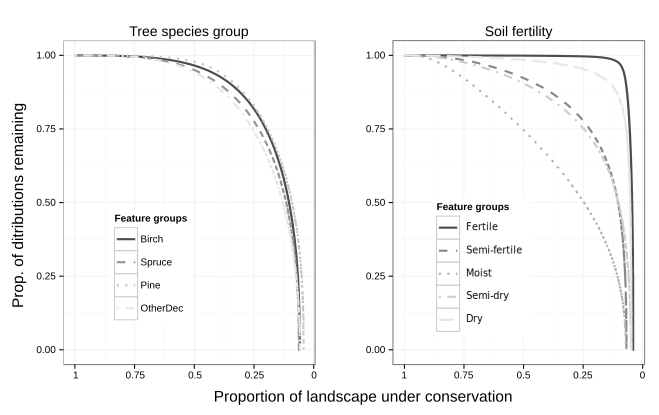
\includegraphics{figs/Fig3.png}
\caption{Figure3}
\end{figure}

\section{Supplementary material}

Building the ecological model Expert elicitation Figure S1: The benefit
functions used to scale the perceived, expert opinion based conservation
value (y-axis) to forest structural characteristics (x-axis)
Segmentation of the MSNFI data

Analysis setup: Table S1: Feature weights Table S2: Connectivity matrix

\end{document}
